%
%  Erik Olsen
%
\documentclass[12pt,fullpage]{article}
\usepackage{fullpage}
\usepackage{amsmath}
\usepackage{psfrag}                                          % LaTeX graphics tool
\usepackage{pslatex}                                         % avoids the default cmr font
\usepackage{graphicx}                                        % graphics package 
\usepackage{epsfig}                                          % figures
\usepackage{hyperref}
\usepackage{color}

\begin{document}

\noindent
{\bf Pascal distribution} (from \color{blue}\url{http://www.math.wm.edu/~leemis/chart/UDR/UDR.html}\color{black})

\noindent
The shorthand $X \sim {\rm Pascal}(n,\, p)$ is used to indicate that the
random variable $X$ has the Pascal distribution positive integer parameter~$n$ and real parameter $p$ satisfying $0<p<1$.
A Pascal random variable $X$ has probability mass function 
$$
f(x) = {{n-1+x} \choose x} \kern 0.08 em p ^ {\kern 0.08 em n} \left(1
- p \right) ^ x \qquad \qquad x = 0,\, 1,\, 2, \ldots .
$$
The Pascal distribution is also known as the negative binomial distribution.
The Pascal distribution can be used to model the number of failures before the 
$n$th success in repeated mutually independent Bernoulli trials, each with probability 
of success $p$.
Applications include acceptance sampling in quality control and modeling demand for a product.
The probability mass function for three different parameter settings is illustrated below.
\begin{figure}[h!]
\begin{center}
\psfrag{labn2}{$n = 2$}
\psfrag{labp25}{$p = 0.25$}
\psfrag{labp5}{$p = 0.5$}
\psfrag{labn5}{$n = 5$}
\psfrag{labx}{$x$}
\psfrag{labf}{$f(x)$}
\includegraphics[width=5.6in]{PascalPlot.ps}
\end{center}
\end{figure}
\\
The cumulative distribution function, survivor function, inverse distribution function, and hazard function of $X$ are mathematically intractable.
The moment generating function of $X$ is
$$
M(t) = E \left[ e ^ {\kern 0.08 em tX} \right] = \left[ \frac {p} {1 - \left( 1 - p \right) e ^ {\kern 0.08 em t}} \right] ^ n
$$
for $|(1 - p)e^t| < 1$ or $t < -\ln (1 - p).$\\ \\
The population mean, variance, skewness, and kurtosis of $X$ are
$$
E[X] = \frac{n(1-p)}{p} \qquad \qquad 
V[X] = \frac{n (1 - p)}{p^2} \qquad \qquad
$$
$$
E\left[ \left( \frac{X - \mu}{\sigma} \right) ^ {\kern -0.08 em 3} \right] =  \frac{2 - p}{\sqrt{n (1 - p)}} \qquad \qquad 
E\left[ \left( \frac{X - \mu}{\sigma} \right) ^ {\kern -0.08 em 4} \right] = \frac{p ^ 2 - 6p - 3np + 3n + 6}{n(1 - p)}.
$$

\vspace{0.1in}

\newpage

\noindent
{\bf APPL verification:}
The APPL statements
\begin{verbatim}
X := NegativeBinomialRV(n, p);
MGF(X);
Variance(X);
Skewness(X);
Kurtosis(X);
\end{verbatim}
verify the moment generating function, population variance, skewness, and kurtosis.

\end{document}
